\documentclass[a4paper,11pt,parskip=half,headings=small,DIV=11,notitlepage,abstract=on]{scrartcl}
% This file contains configuration shared between main file and figures

\usepackage{pifont}
\usepackage{xspace}
\DeclareUnicodeCharacter{2460}{\ding{172}\xspace}
\DeclareUnicodeCharacter{2461}{\ding{173}\xspace}

\usepackage{tikz}

\definecolor{HB9UFblue}{RGB}{0,61,165}
\definecolor{HB9UFred}{HTML}{ED135A}

\newcommand{\Ohm}{$\Omega$\xspace}


\newcommand{\uline}[1]{%
  \tikz[baseline=(todotted.base)]{
      \node[inner sep=1pt,outer sep=0pt] (todotted) {#1};
      \draw[color=HB9UFblue,thick] (todotted.south west) -- (todotted.south east);
  }%
}%
                           
\newcommand{\udash}[1]{%
  \tikz[baseline=(todotted.base)]{
      \node[inner sep=1pt,outer sep=0pt] (todotted) {#1};
      \draw[dashed,color=HB9UFred,thick] (todotted.south west) -- (todotted.south east);
  }%
}%

\usepackage{scrlayer-scrpage}
\usepackage{graphicx}
\usepackage{amsmath}
\usepackage[pdfauthor={},pdftitle={},pdfstartview=FitH,pdfborder={0 0 0}]{hyperref}
\usepackage[utf8]{inputenc}
\usepackage{textcomp}
\usepackage{booktabs}
\renewcommand{\thesection}{\Alph{section}}
\renewcommand*{\theenumi}{\thesection.\arabic{enumi}}

\usepackage{ngerman}
\ifoot{\texttt{}}
\ofoot{\texttt{}}

%\addtolength{\textheight}{5mm}
\title{Posten D\\Antennen}
\author{}
\date{}
\pagestyle{empty}
\renewcommand*{\titlepagestyle}{empty}
\sloppy

\begin{document}
\maketitle
\vspace{-2cm}
An diesem Posten geht es um das Charakterisieren von Antennen. Folgendes
vorweg: Der VNA kann nicht abschliessend beurteilen, wie ``gut'' eine Antenne
ist. Es geht lediglich darum zu prüfen, ob eine Antenne die richtige Impedanz
aufweist, um die zugeführte Leistung aufnehmen zu können. Ob diese Leistung
dann in die richtige oder in eine unerwünschte Richtig abgestrahlt, in den
Boden eingekoppelt oder einfach verheizt wird, dann das Gerät nicht beurteilen.
Das Einkoppeln der Leistung ist aber eine Voraussetzung, damit diese in Form
von Funkwellen abgestrahlt werden kann.

Dies erfolgt mit einer Reflexionsmessung, als Trace-Formal wählt man ``LogMag'', um die
Resultate als Rückführungsdämpfung anzuzeigen, oder ``SWR'' für die Angabe des
Stehwellenverhältnis. Es ist aber auch möglich, sich einen Überblick über Wirk-
und Blindanteile der Antennenimpedanz zu verschaffen, beispielsweise mit dem
Smith-Diagramm. In diesem Fall ist eine Kalibrierung am Fusspunkt besonders wichtig,
da die Speiseleitung diese Impedanzen ansonsten transformieren würde. Im Skript
findest du eine Tabelle, welche Einsicht in den Zusammenhang zwischen SWR,
Rückführungsdämpfung und den Prozentanteil der reflektierten Leistung gibt.

Die Antenne wird möglichst direkt (z.B. mit einem kurzen Messkabel) mit dem
VNA verbunden, die Kalibrierung erfolgt idealerweise am Antennenfusspunkt:

\begin{center}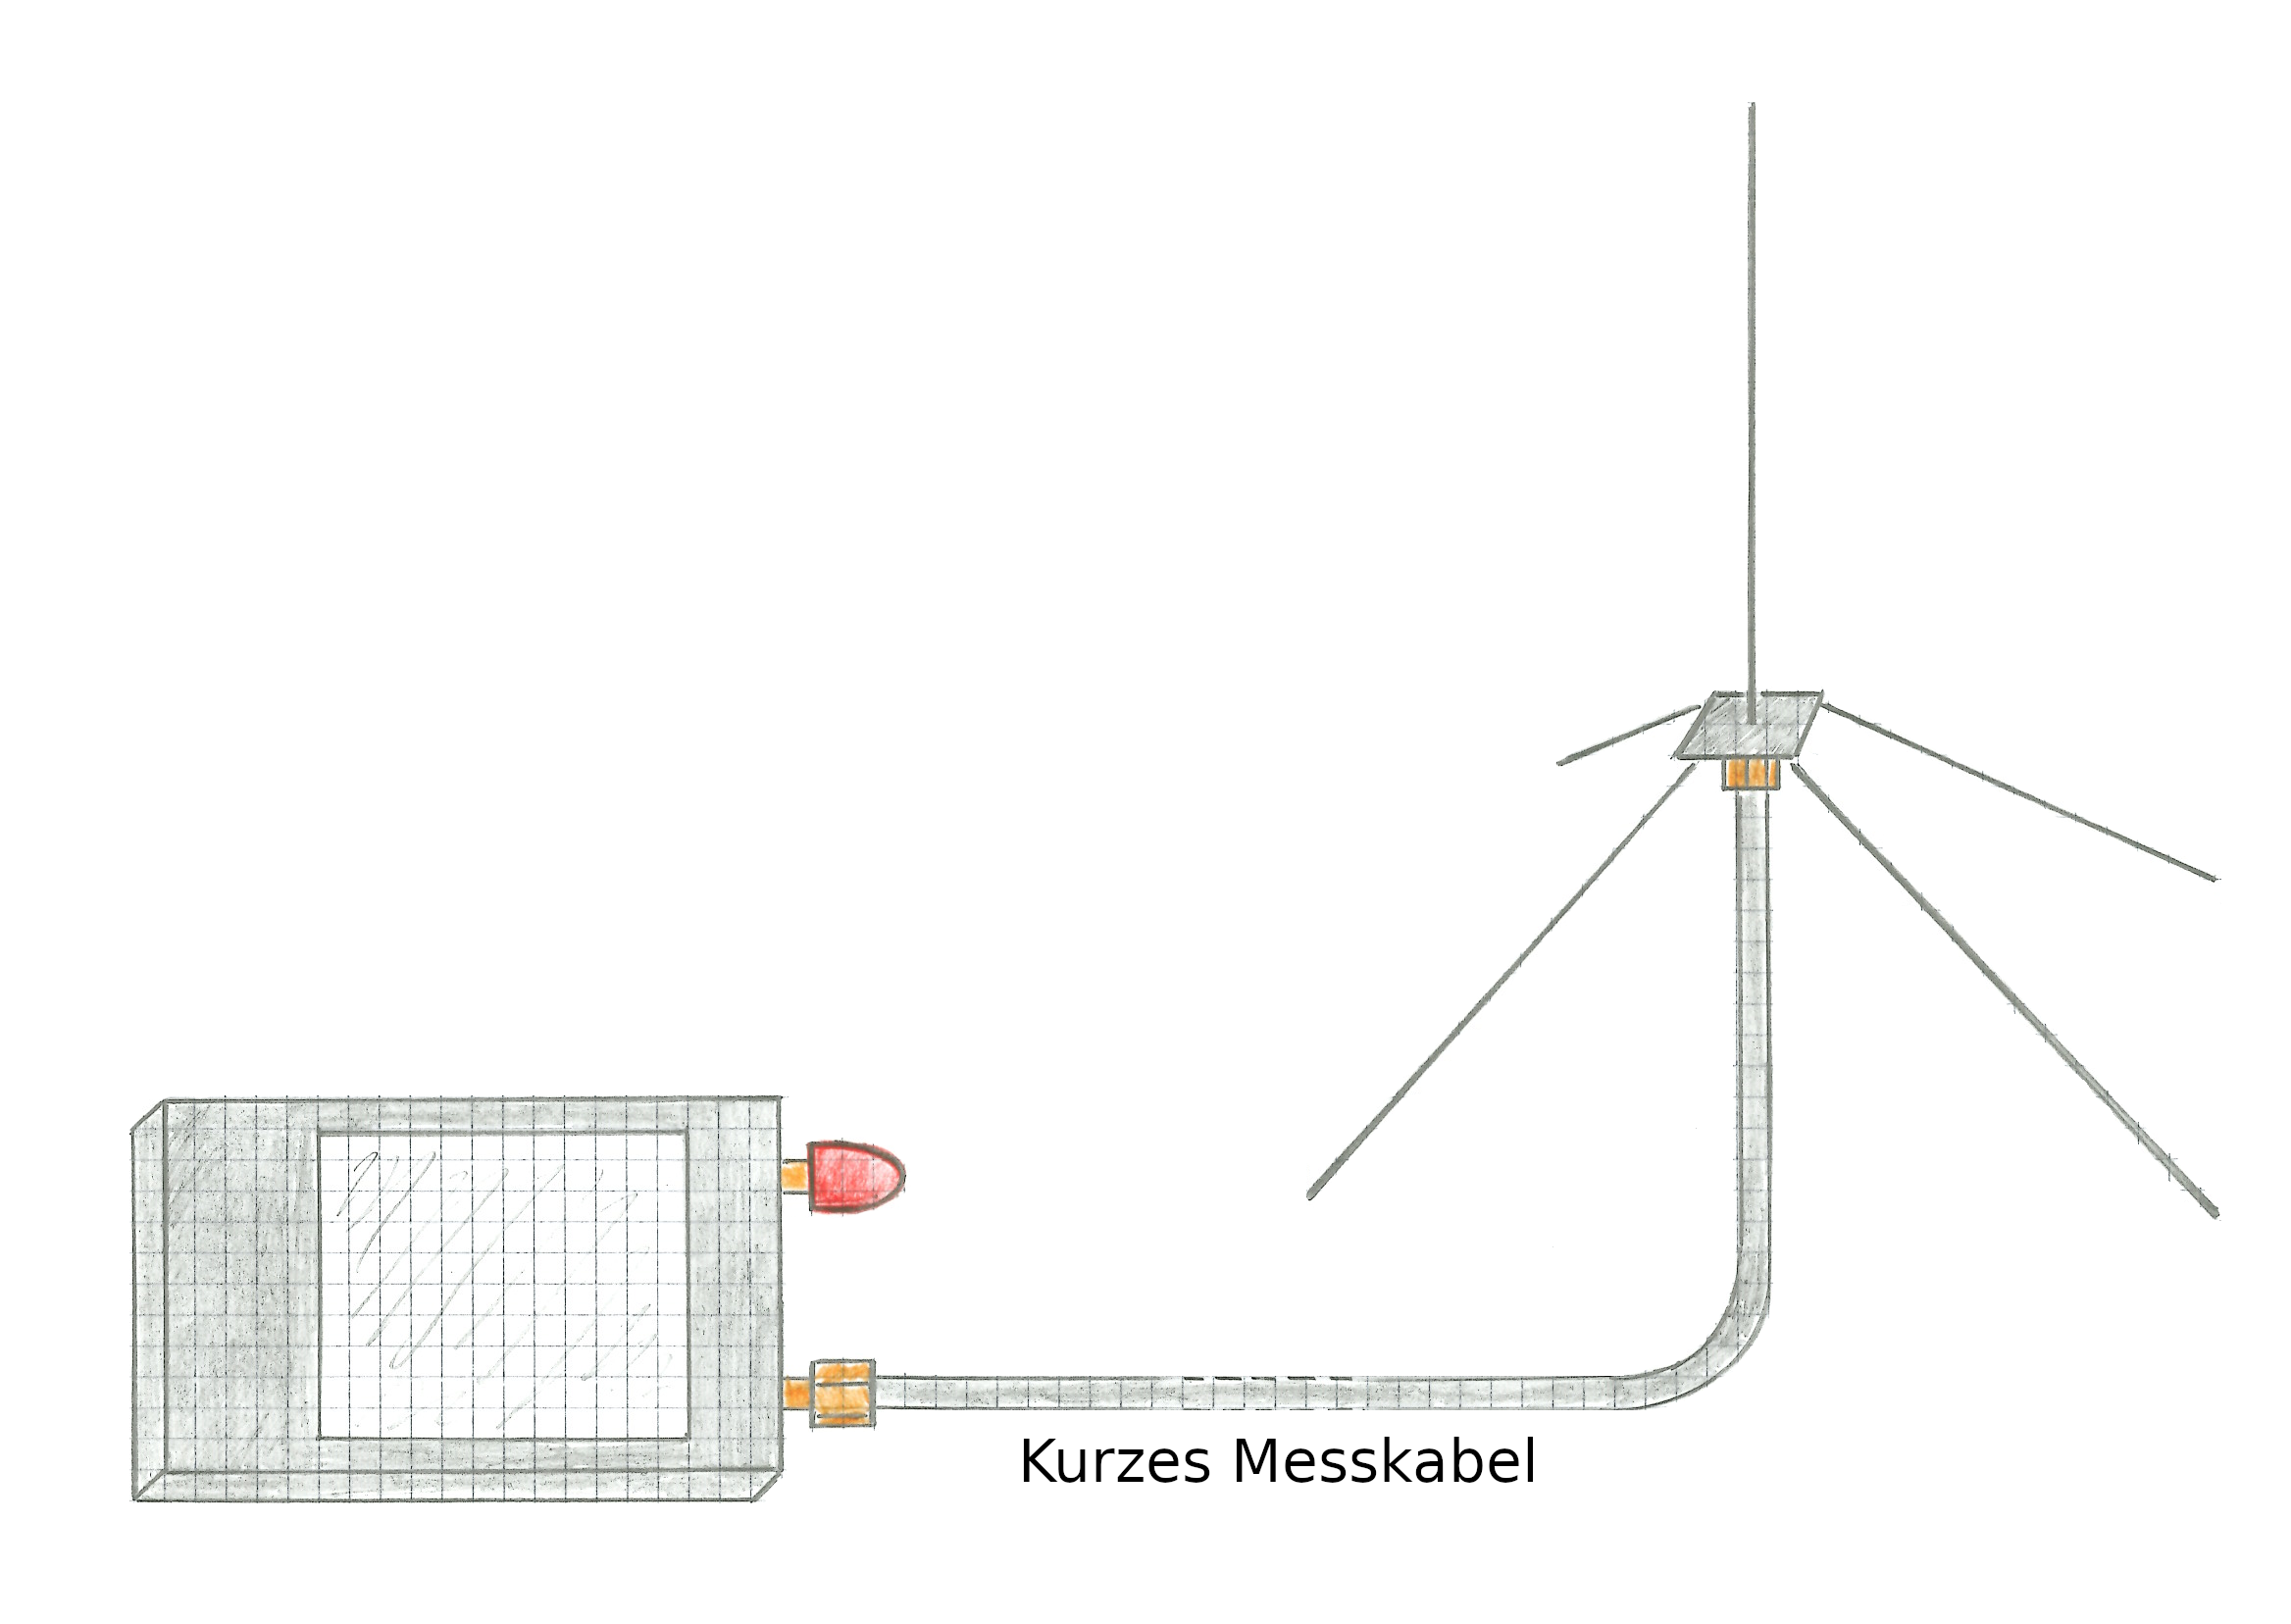
\includegraphics[width=0.7\textwidth]{../skript/figures/illustration_antenna.png}\end{center}

Grundsätzlich ist es auch möglich, den Einfluss der Speiseleitung mitzumessen.
Die folgende Abbildung zeigt einen Vergleich zwischen der Messung einer VHF/UHF
Zweibandantenne direkt am Antennefusspunkt (ausgezogene Linie) und einer Messung
derselben Antenne, aber einschliesslich einer 10~m langen Speiseleitung aus
RG-213:

\begin{center}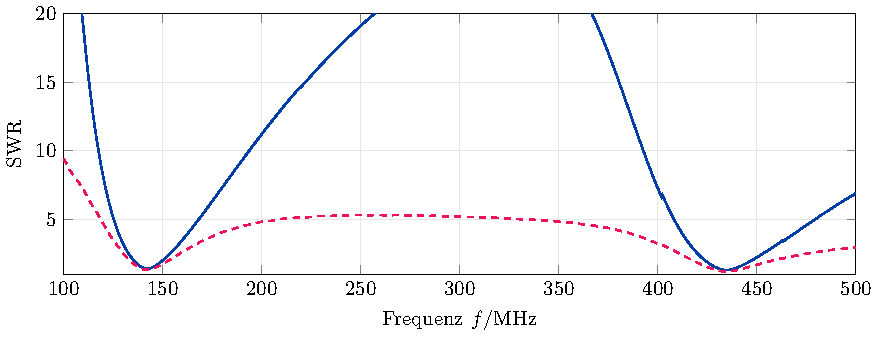
\includegraphics{../skript/figures/feednofeed/feednofeed.pdf}\end{center}  

Die Kalibrierung erfolgte dabei jeweils direkt am Port. Hier wird ersichtlich,
dass die reflektierte Leistung durch die Kabeldämpfung in Wärme umgewandelt
wird. Es kommt beim VNA deshalb nur ein Teil dieser reflektierten Leistung an,
das SWR dieses Antennensystems ist ``besser'' als dasjenige der Antenne alleine.
Ein Bewusstsein für diesen Sachverhalt vermeidet hier Fehlinterpretationen. Eine
Kalibrierung am Antennen-Ende der Speiseleitung würde, in der Theorie, diesen
Effekt kompensieren.

Unten ist ein einfaches Antennenmodell gezeigt -- im Wesentlichen handelt es
sich um einen Serienschwingkreis. Unterhalb der Resonanzfrequenz ist die Antenne
kapazitiv (der Bilindwiderstand der Kapazität dominiert), oberhalb der Resonanzfrequenz
ist die Antenne induktiv (der Blindwiderstand der Induktivität dominiert). Genau
bei Resonanz heben sich die beiden Blindwiderstände auf, der VNA sieht nur den
Widerstand $R_\text{strahl}+R_\text{ohm}$. Das SWR wird dann durch das Verhältnis
dieses Widerstandes zur Systemimpedanz bestimmt.

  \begin{center}
      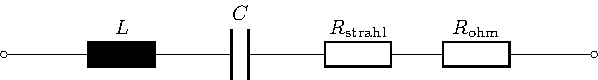
\includegraphics{../skript/figures/antenna_model/antenna_model.pdf}
  \end{center}

Zum Praktizieren dieser Messung haben wir eine Rahmenantenne für das 2~m und das
70~cm Band, eine Doppelquad-Antenne für das 23~cm Band, eine verstellbare
Teleskopantenne und einen Antennenfuss mit SMA-Anschluss mitgebracht. Messe
diese Antennen aus. Achte dabei auch auf den Einfluss von Gegenständen und
Gewebe im Nahfeld der Antenne. Welche NanoVNA-Version schafft auf 1.3~MHz eine
sinnvolle Messung?

\end{document}
